% questions.tex —— 2009 年·普通高等学校招生考试·四川卷·理科 · 题目内容片段（无答案）
% 由 tools/generate_projects.py 依来源总账自 2009/2009_数学真题_四川理_试题.md 生成，勿手改（改源 MD 后重跑）


状态：needs-review；依固定候选 PDF 两页（印刷页 557–558）逐题核验，图形已矢量重绘，正式构建与逐页验收见回执。源未标分值，不补分值。第 11 题四个选项印作 $360$、$188$、$216$、$96$，而按题设算得 $288$，无一相符，照原页保留并登记问题。第 20 题椭圆方程分母印作 $y^2/b$（非 $b^2$），照原页保留。

\gkpart{一、选择题}

\begin{question}
\gkti{1}设集合 $S=\{x\mid |x|<5\}$，$T=\{x\mid x^2+4x-21<0\}$，则 $S\cap T=$（　）

（A）$\{x\mid -7<x<-5\}$

（B）$\{x\mid 3<x<5\}$

（C）$\{x\mid -5<x<3\}$

（D）$\{x\mid -7<x<5\}$

\end{question}
\begin{question}
\gkti{2}已知函数 $f(x)=\begin{cases}a+\log_2x,&x\geqslant2,\\[4pt] \dfrac{x^2-4}{x-2},&x<2\end{cases}$ 在点 $x=2$ 处连续，则常数 $a$ 的值是（　）

（A）$2$

（B）$3$

（C）$4$

（D）$5$

\end{question}
\begin{question}
\gkti{3}复数 $\dfrac{(1+2\mathrm i)^2}{3-4\mathrm i}$ 的值是（　）

（A）$-1$

（B）$1$

（C）$-\mathrm i$

（D）$\mathrm i$

\end{question}
\begin{question}
\gkti{4}已知函数 $f(x)=\sin\left(x-\dfrac{\pi}{2}\right)$（$x\in\mathbf R$），下面结论错误的是（　）

（A）函数 $f(x)$ 的最小正周期为 $2\pi$

（B）函数 $f(x)$ 在区间 $\left[0,\dfrac{\pi}{2}\right]$ 上是增函数

（C）函数 $f(x)$ 的图象关于直线 $x=0$ 对称

（D）函数 $f(x)$ 是奇函数

\Needspace{0.4\textheight}
\end{question}
\begin{question}
\gkti{5}如图，已知六棱锥 $P-ABCDEF$ 的底面是正六边形，$PA\perp$ 平面 $ABC$，$PA=2AB$，则下列结论正确的是（　）
\nopagebreak[4]
\begin{center}% 2009 年四川卷理科第 5 题：题图。
% 来源 PDF：普通高考/2009/2009四川理.pdf，SHA256 7f64be22c7f7c29a749b276635494972f962f91302ebc7506b55c9fae85a7406
% 原页：第 1 页（A3 三栏）第 1 栏中部，印刷页 557。
% 重绘依据：正六棱锥 P-ABCDEF，PA⊥底面，PA=2AB；与文科第 6 题同图。
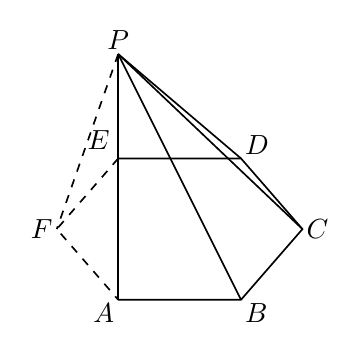
\begin{tikzpicture}[scale=0.78, semithick, every node/.style={inner sep=1.2pt}]
  \coordinate (A) at (0,0);
  \coordinate (B) at (2,0);
  \coordinate (C) at (3,1.15);
  \coordinate (D) at (2,2.3);
  \coordinate (E) at (0,2.3);
  \coordinate (F) at (-1,1.15);
  \coordinate (P) at (0,4.0);
  \draw[dashed] (E) -- (F) -- (A);
  \draw (A) -- (B) -- (C) -- (D) -- (E);
  \draw (P) -- (A);
  \draw (P) -- (B);
  \draw (P) -- (C);
  \draw (P) -- (D);
  \draw[dashed] (P) -- (E);
  \draw[dashed] (P) -- (F);
  \node[anchor=south] at (P) {$P$};
  \node[anchor=north east] at (A) {$A$};
  \node[anchor=north west] at (B) {$B$};
  \node[anchor=west] at (C) {$C$};
  \node[anchor=south west] at (D) {$D$};
  \node[anchor=south east] at ([xshift=-2pt,yshift=2pt]E) {$E$};
  \node[anchor=east] at (F) {$F$};
\end{tikzpicture}
\end{center}
\nopagebreak[4]
（A）$PB\perp AD$

（B）平面 $PAB\perp$ 平面 $PBC$

（C）直线 $BC\parallel$ 平面 $PAE$

（D）直线 $PD$ 与平面 $ABC$ 所成的角为 $45^\circ$

\end{question}
\begin{question}
\gkti{6}已知 $a,b,c,d$ 为实数，且 $c>d$．则「$a>b$」是「$a-c>b-d$」的（　）

（A）充分而不必要条件

（B）必要而不充分条件

（C）充要条件

（D）既不充分也不必要条件

\end{question}
\begin{question}
\gkti{7}已知双曲线 $\dfrac{x^2}{2}-\dfrac{y^2}{b^2}=1$（$b>0$）的左、右焦点分别为 $F_1,F_2$，其一条渐近线方程为 $y=x$，点 $P(\sqrt3,y_0)$ 在该双曲线上，则 $\overrightarrow{PF_1}\cdot\overrightarrow{PF_2}=$（　）

（A）$-12$

（B）$-2$

（C）$0$

（D）$4$

\Needspace{0.4\textheight}
\end{question}
\begin{question}
\gkti{8}如图，在半径为 $3$ 的球面上有 $A,B,C$ 三点，$\angle ABC=90^\circ$，$BA=BC$，球心 $O$ 到平面 $ABC$ 的距离是 $\dfrac{3\sqrt2}{2}$，则 $B,C$ 两点的球面距离是（　）
\nopagebreak[4]
\begin{center}% 2009 年四川卷理科第 8 题：题图。
% 来源 PDF：普通高考/2009/2009四川理.pdf，SHA256 7f64be22c7f7c29a749b276635494972f962f91302ebc7506b55c9fae85a7406
% 原页：第 1 页（A3 三栏）第 2 栏上部，印刷页 557。
% 重绘依据：球面三点 A、B、C，∠ABC=90°，BA=BC；与文科第 9 题同图。
\begin{tikzpicture}[scale=1.2, semithick, every node/.style={inner sep=1.2pt}]
  \coordinate (O) at (0,0);
  \draw (O) circle (2);
  \fill (O) circle (1.2pt);
  \node[anchor=south west] at ($(O)+(0.13,0.11)$) {$O$};
  \coordinate (A) at (135:1.35);
  \coordinate (B) at (215:1.35);
  \coordinate (C) at (305:1.35);
  \draw (A) -- (B) -- (C) -- (A);
  \draw[dashed] (O) -- (A);
  \draw[dashed] (O) -- (B);
  \draw[dashed] (O) -- (C);
  \node[anchor=south east] at (A) {$A$};
  \node[anchor=north east] at (B) {$B$};
  \node[anchor=north west] at (C) {$C$};
\end{tikzpicture}
\end{center}
\nopagebreak[4]
（A）$\dfrac{\pi}{3}$

（B）$\pi$

（C）$\dfrac{4\pi}{3}$

（D）$2\pi$

\end{question}
\begin{question}
\gkti{9}已知直线 $l_1:4x-3y+6=0$ 和直线 $l_2:x=-1$，抛物线 $y^2=4x$ 上一动点 $P$ 到直线 $l_1$ 和直线 $l_2$ 的距离之和的最小值是（　）

（A）$2$

（B）$3$

（C）$\dfrac{11}{5}$

（D）$\dfrac{37}{16}$

\end{question}
\begin{question}
\gkti{10}某企业生产甲、乙两种产品，已知生产每吨甲产品要用 A 原料 $3$ 吨、B 原料 $2$ 吨；生产每吨乙产品要用 A 原料 $1$ 吨、B 原料 $3$ 吨．销售每吨甲产品可获得利润 $5$ 万元，每吨乙产品可获得利润 $3$ 万元，该企业在一个生产周期内消耗 A 原料不超过 $13$ 吨，B 原料不超过 $18$ 吨，那么该企业可获得最大利润是（　）

（A）$12$ 万元

（B）$20$ 万元

（C）$25$ 万元

（D）$27$ 万元

\end{question}
\begin{question}
\gkti{11}$3$ 位男生和 $3$ 位女生共 $6$ 位同学站成一排，若男生甲不站两端，$3$ 位女生中有且只有两位女生相邻，则不同排法的种数是（　）

（A）$360$

（B）$188$

（C）$216$

（D）$96$

\end{question}
\begin{question}
\gkti{12}已知函数 $f(x)$ 是定义在实数集 $\mathbf R$ 上的不恒为零的偶函数，且对任意实数 $x$ 都有 $xf(x+1)=(1+x)f(x)$，则 $f\left(f\left(\dfrac52\right)\right)$ 的值是（　）

（A）$0$

（B）$\dfrac12$

（C）$1$

（D）$\dfrac52$

\end{question}
\gkpart{二、填空题}

\begin{question}
\gkti{13}$\left(2x-\dfrac1{2x}\right)^6$ 的展开式的常数项是\gkblank{}．（用数字作答）

\end{question}
\begin{question}
\gkti{14}若 $\odot O_1:x^2+y^2=5$ 与 $\odot O_2:(x-m)^2+y^2=20$（$m\in\mathbf R$）相交于 $A,B$ 两点，且两圆在点 $A$ 处的切线互相垂直，则线段 $AB$ 的长度是\gkblank{}．

\Needspace{0.4\textheight}
\end{question}
\begin{question}
\gkti{15}如图，已知正三棱柱 $ABC-A_1B_1C_1$ 的各条棱长都相等，$M$ 是侧棱 $CC_1$ 的中点，则异面直线 $AB_1$ 和 $BM$ 所成的角的大小是\gkblank{}．
\nopagebreak[4]
\begin{center}% 2009 年四川卷理科第 15 题：题图。
% 来源 PDF：普通高考/2009/2009四川理.pdf，SHA256 7f64be22c7f7c29a749b276635494972f962f91302ebc7506b55c9fae85a7406
% 原页：第 1 页（A3 三栏）第 2 栏下部，印刷页 557。
% 重绘依据：各棱长都相等的正三棱柱，M 为 CC_1 中点；与文科第 15 题同图。
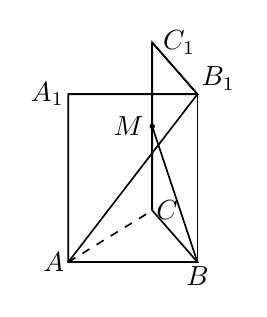
\begin{tikzpicture}[scale=0.82, semithick, every node/.style={inner sep=1.2pt}]
  \coordinate (A) at (0,0);
  \coordinate (B) at (2,0);
  \coordinate (C) at (1.3,0.8);
  \coordinate (A1) at (0,2.6);
  \coordinate (B1) at (2,2.6);
  \coordinate (C1) at (1.3,3.4);
  \coordinate (M) at (1.3,2.1);
  \draw[dashed] (A) -- (C);
  \draw (A) -- (B) -- (C) -- (C1) -- (B1) -- (A1) -- cycle;
  \draw (B) -- (B1);
  \draw (C) -- (C1);
  \draw (A1) -- (B1);
  \draw (B1) -- (C1);
  \draw (A) -- (B1);
  \draw (B) -- (M);
  \fill (M) circle (1.2pt);
  \node[anchor=east] at (A) {$A$};
  \node[anchor=north] at (B) {$B$};
  \node[anchor=west] at (C) {$C$};
  \node[anchor=east] at (A1) {$A_1$};
  \node[anchor=south west] at (B1) {$B_1$};
  \node[anchor=west] at ([xshift=3pt]C1) {$C_1$};
  \node[anchor=east] at ([xshift=-2pt]M) {$M$};
\end{tikzpicture}
\end{center}
\nopagebreak[4]
\end{question}
\begin{question}
\gkti{16}设 $V$ 是已知平面 $M$ 上所有向量的集合，对于映射 $f:V\to V$，$\boldsymbol a\in V$，记 $\boldsymbol a$ 的象为 $f(\boldsymbol a)$．若映射 $f:V\to V$ 满足：对所有 $\boldsymbol a,\boldsymbol b\in V$ 及任意实数 $\lambda,\mu$ 都有 $f(\lambda\boldsymbol a+\mu\boldsymbol b)=\lambda f(\boldsymbol a)+\mu f(\boldsymbol b)$，则 $f$ 称为平面 $M$ 上的线性变换．现有下列命题：

① 设 $f$ 是平面 $M$ 上的线性变换，则 $f(\boldsymbol 0)=\boldsymbol 0$；

② 对 $\boldsymbol a\in V$，设 $f(\boldsymbol a)=2\boldsymbol a$，则 $f$ 是平面 $M$ 上的线性变换；

③ 若 $\boldsymbol e$ 是平面 $M$ 上的单位向量，对 $\boldsymbol a\in V$，设 $f(\boldsymbol a)=\boldsymbol a-\boldsymbol e$，则 $f$ 是平面 $M$ 上的线性变换；

④ 设 $f$ 是平面 $M$ 上的线性变换，$\boldsymbol a,\boldsymbol b\in V$，若 $\boldsymbol a,\boldsymbol b$ 共线，则 $f(\boldsymbol a),f(\boldsymbol b)$ 也共线．

其中真命题是\gkblank{}．（写出所有真命题的序号）

\end{question}
\gkpart{三、解答题}

\begin{question}
\gkti{17}在 $\triangle ABC$ 中，$A,B$ 为锐角，角 $A,B,C$ 所对的边分别为 $a,b,c$，且 $\cos2A=\dfrac35$，$\sin B=\dfrac{\sqrt{10}}{10}$．

（1）求 $A+B$ 的值；

（2）若 $a-b=\sqrt2-1$，求 $a,b,c$ 的值．

\end{question}
\begin{question}
\gkti{18}为振兴旅游业，四川省 2009 年面向国内发行总量为 $2000$ 万张的熊猫优惠卡，向省外人士发行的是熊猫金卡（简称金卡），向省内人士发行的是熊猫银卡（简称银卡）．某旅游公司组织了一个有 $36$ 名游客的旅游团到四川名胜旅游，其中 $\dfrac34$ 是省外游客，其余是省内游客．在省外游客中有 $\dfrac13$ 持金卡，在省内游客中有 $\dfrac23$ 持银卡．

（1）在该团中随机采访 $3$ 名游客，求恰有 $1$ 人持金卡且持银卡者少于 $2$ 人的概率；

（2）在该团的省内游客中随机采访 $3$ 名游客，设其中持银卡人数为随机变量 $\xi$，求 $\xi$ 的分布列及数学期望 $E\xi$．

\Needspace{0.4\textheight}
\end{question}
\begin{question}
\gkti{19}如图，正方形 $ABCD$ 所在平面与平面四边形 $ABEF$ 所在平面互相垂直，$\triangle ABE$ 是等腰直角三角形，$AB=AE$，$FA=FE$，$\angle AEF=45^\circ$．
\nopagebreak[4]
\begin{center}% 2009 年四川卷理科第 19 题：正方形 ABCD 与平面四边形 ABEF 所在平面互相垂直。
% 来源 PDF：普通高考/2009/2009四川理.pdf，SHA256 7f64be22c7f7c29a749b276635494972f962f91302ebc7506b55c9fae85a7406
% 原页：第 2 页（A3 三栏）第 1 栏中部，印刷页 558。
% 重绘依据：按原图取 A 左上、B 右上、C 右下、D 左下（斜投影平行四边形）；ABEF 为竖直平面，
%   E 在 A 正上方、F 在 A 的左上方，FA=FE；AB 被平面 ABEF 遮挡画虚线；
%   辅助线 EC、DB 与正方形边 AD、DC、CB 实线；P 为 DC 中点。第 (2) 问的 M 待求，图上不画。
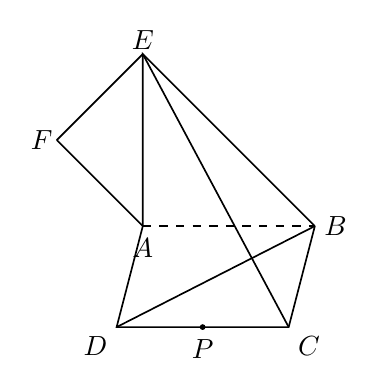
\begin{tikzpicture}[scale=0.95, semithick, every node/.style={inner sep=1.2pt}]
  \coordinate (A) at (0,0);
  \coordinate (B) at (2.3,0);
  \coordinate (C) at (1.95,-1.35);
  \coordinate (D) at (-0.35,-1.35);
  \coordinate (E) at (0,2.3);
  \coordinate (F) at (-1.15,1.15);
  \coordinate (P) at (0.8,-1.35);
  % 正方形（AB 被遮挡）
  \draw[dashed] (A) -- (B);
  \draw (B) -- (C) -- (D) -- (A);
  % 四边形 ABEF
  \draw (A) -- (E) -- (B);
  \draw (F) -- (A);
  \draw (F) -- (E);
  % 辅助线
  \draw (E) -- (C);
  \draw (D) -- (B);
  % 中点 P
  \fill (P) circle (1.1pt);
  \node[anchor=north] at ([yshift=-3pt]A) {$A$};
  \node[anchor=west] at ([xshift=2pt]B) {$B$};
  \node[anchor=north west] at ([xshift=2pt,yshift=-2pt]C) {$C$};
  \node[anchor=north east] at ([xshift=-2pt,yshift=-2pt]D) {$D$};
  \node[anchor=south] at (E) {$E$};
  \node[anchor=east] at (F) {$F$};
  \node[anchor=north] at ([yshift=-3pt]P) {$P$};
\end{tikzpicture}
\end{center}
\nopagebreak[4]
（1）求证：$EF\perp$ 平面 $BCE$；

（2）设线段 $CD$ 的中点为 $P$，在直线 $AE$ 上是否存在一点 $M$，使得 $PM\parallel$ 平面 $BCE$？若存在，请指出点 $M$ 的位置，并证明你的结论；若不存在，请说明理由；

（3）求二面角 $F-BD-A$ 的大小．

\end{question}
\begin{question}
\gkti{20}已知椭圆 $\dfrac{x^2}{a^2}+\dfrac{y^2}{b}=1$（$a>b>0$）的左、右焦点分别为 $F_1,F_2$，离心率 $e=\dfrac{\sqrt2}{2}$，右准线方程为 $x=2$．

（1）求椭圆的标准方程；

（2）过点 $F_1$ 的直线 $l$ 与该椭圆交于 $M,N$ 两点，且 $\left|\overrightarrow{F_2M}+\overrightarrow{F_2N}\right|=\dfrac{2\sqrt{26}}{3}$，求直线 $l$ 的方程．

\end{question}
\begin{question}
\gkti{21}已知 $a>0$，且 $a\neq1$，函数 $f(x)=\log_a(1-a^x)$．

（1）求函数 $f(x)$ 的定义域，并判断 $f(x)$ 的单调性；

（2）若 $n\in\mathbf N^*$，求 $\lim\limits_{n\to\infty}\dfrac{a^{f(n)}}{a^n+a}$；

（3）当 $a=\mathrm e$（$\mathrm e$ 为自然对数的底数）时，设 $h(x)=(1-\mathrm e^{f(x)})(x^2-m+1)$．若函数 $h(x)$ 的极值存在，求实数 $m$ 的取值范围以及函数 $h(x)$ 的极值．

\end{question}
\begin{question}
\gkti{22}设数列 $\{a_n\}$ 的前 $n$ 项和为 $S_n$，对任意的正整数 $n$，都有 $a_n=5S_n+1$ 成立，记 $b_n=\dfrac{4+a_n}{1-a_n}$（$n\in\mathbf N^*$）．

（1）求数列 $\{b_n\}$ 的通项公式；

（2）记 $c_n=b_{2n}-b_{2n-1}$（$n\in\mathbf N^*$），设数列 $\{c_n\}$ 的前 $n$ 项和为 $T_n$，求证：对任意正整数 $n$ 都有 $T_n<\dfrac32$；

（3）设数列 $\{b_n\}$ 的前 $n$ 项和为 $R_n$．已知正实数 $\lambda$ 满足：对任意正整数 $n$，$R_n\leqslant\lambda n$ 恒成立，求 $\lambda$ 的最小值．

\end{question}